\chapter{Research Questions} \label{rq}

In this chapter we will present some possible research areas for systematic reviews.

\section{Automated Decision Making of Relevant Studies} \label{dm}

Once relevant studies have been identified by their abstracts, reviewers are required to process the studies and extract useful information for the systematic review. Many of these studies will not be useful and can be discarded, but not without the cost of the reviewer having to look at the content.

A useful piece of research would be to determine if a study is relevant to the systematic review question. 

There are two potential routes that could be taken for the investigating this task. The first approach would be to use existing information from the systematic review (ie the protocol) and determine if the study contains the information. A second approach would be to a semi-supervised learning method, having the reviewer look at a subset of the studies, so we can then build a classifier for the remaining studies. Both of these approaches can be applied to the abstract screening and the data filtering stage of the systematic review. For the abstract screening we would be trying to predict if a study is relevant, by looking at the abstract. For the data filtering stage we would be looking at the actual text of the study (typically a pdf file)

There are many challenges for this research topic. Not all studies are publicly available and are often protected by publishing licences. This makes it difficult to gather data. Another challenge is having to deal with such a broad range of data, as well as the pdf format studies.

\section{Information Extraction From Studies} \label{ie}

In a similar vein to the first topic \ref{dm} we could also look at extracting the relevant information from a study. Often empirical data is identified in studies and extracted to generate a tree diagram:

\begin{figure}[H]
\center
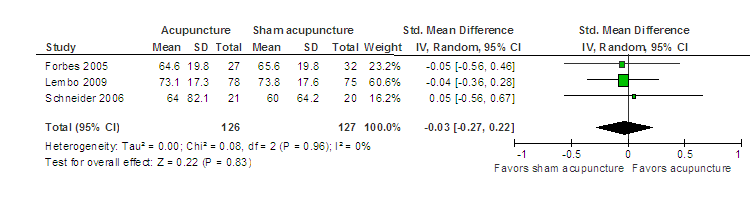
\includegraphics[width=16cm]{figures/tree.png}
\caption{Tree diagram example, all credit for diagram goes here \cite{Manheimer2012}}
\end{figure}

These tree diagrams contain summarized information from the relevant studies. Studies that contain more useful (i.e higher number of participants) have smaller confidence margins and vice-versa for smaller studies.

An interesting area of research would be identifying empirical data in a study to generate these tree diagrams automatically.

The challenge in this task is gathering training data that is sufficiently marked as to where key information occurs within a study. This would would also still involve working with a limited number of studies and pdf documents.

\section{Stopping Methods} \label{sm}

We examined existing working on finding on stopping methods in our literature survey \ref{stops}. We can investigate further methods finding stopping points in systematic review rankings. 

We can look at applying machine learning algorithms for plotting a regression based system of relevant documents. Techniques that could be interesting to experiment with include a generic curve fitting and a Gaussian Process (GP).
